\documentclass[12pt,a4paper]{article}
\usepackage[utf8]{inputenc}
\usepackage[margin=1in]{geometry}
\usepackage{graphicx}
\usepackage{amsmath}
\usepackage{amsfonts}
\usepackage{amssymb}
\usepackage{hyperref}
\usepackage{listings}
\usepackage{xcolor}
\usepackage{fancyhdr}
\usepackage{titlesec}
\usepackage{tocloft}
\usepackage{float}
\usepackage{natbib}
\usepackage{tikz}
\usetikzlibrary{shapes,arrows,positioning}
\usepackage{pgfplots}
\pgfplotsset{compat=1.18}

\title{CyberGuard: A Comprehensive Cybercrime Prevention and Reporting Web Application}
\author{Priyanshu Kumar Sharma}
\date{\today}

\pagestyle{fancy}
\fancyhf{}
\rhead{CyberGuard Project Report}
\lhead{CFIS - SEM 7}
\cfoot{\thepage}

\begin{document}

\maketitle

\newpage
\begin{abstract}
Cybercrime has emerged as one of the most significant threats in our digital society, with damages projected to reach \$10.5 trillion annually by 2025. Traditional cybercrime reporting mechanisms often involve complex bureaucratic processes that discourage victims from reporting incidents. This project presents CyberGuard, a comprehensive web-based cybercrime prevention and reporting system designed to bridge the gap between cybercrime victims and law enforcement agencies.

The system implements a three-tier architecture using Node.js, Express.js, and responsive frontend technologies to deliver a secure, user-friendly platform. Key features include role-based access control, comprehensive incident reporting with evidence attachment capabilities, real-time case tracking, and educational resources for cybersecurity awareness. The application supports multiple cybercrime categories including phishing, identity theft, financial fraud, cyberbullying, and ransomware attacks.

Security measures include bcrypt password hashing, input validation following OWASP guidelines, secure file upload mechanisms, and session management with HTTP-only cookies. The system is deployed on cloud infrastructure using Render.com, providing scalability and high availability for public access.

Testing encompasses functional, security, performance, and usability evaluation, demonstrating the system's effectiveness in serving both technical and non-technical users. The implementation successfully addresses accessibility barriers, provides transparency in case progress, and offers comprehensive evidence collection guidance.

Results show that the system achieves sub-2-second response times, handles concurrent users effectively, and maintains security standards for sensitive data protection. User experience evaluation confirms intuitive navigation and successful task completion across various devices and user skill levels.

The project contributes to cybersecurity infrastructure by providing an accessible reporting platform that encourages incident documentation while supporting effective case management for law enforcement. Future enhancements include mobile applications, advanced analytics, and integration with external cybersecurity systems.
\end{abstract}

\newpage
\tableofcontents
\newpage

\section{Executive Summary}

The CyberGuard project represents a comprehensive web-based solution designed to address the growing concerns of cybercrime in our digital society. This application serves as a centralized platform where citizens can report cybercrime incidents, track their case progress, and access valuable prevention resources. The system incorporates modern web technologies including Node.js, Express.js, and responsive frontend design to deliver a secure, user-friendly experience.

The primary objective of this project is to bridge the gap between cybercrime victims and law enforcement agencies by providing an accessible, secure, and efficient reporting mechanism. The application features role-based access control, comprehensive incident management, and educational resources to empower users with cybersecurity knowledge.

Key achievements include the successful implementation of a full-stack web application with robust security measures, deployment on cloud infrastructure, and creation of an intuitive user interface that accommodates both technical and non-technical users. The system supports multiple types of cybercrime reporting, evidence attachment capabilities, and administrative tools for case management.

\section{Introduction}

\subsection{Background and Motivation}

In the contemporary digital landscape, cybercrime has emerged as one of the most significant threats to individuals, businesses, and governments worldwide. The rapid digitization of services, accelerated by global events such as the COVID-19 pandemic, has created new vulnerabilities and attack vectors that cybercriminals exploit with increasing sophistication.

According to recent statistics from cybersecurity organizations, cybercrime damages are projected to reach \$10.5 trillion annually by 2025 \citep{morgan2020cybersecurity}, with financial losses running into trillions of dollars annually. The types of cybercrimes have evolved from simple email scams to complex multi-stage attacks involving social engineering, advanced persistent threats, and sophisticated malware campaigns.

Traditional reporting mechanisms for cybercrime often involve complex bureaucratic processes, multiple agencies, and lengthy procedures that discourage victims from reporting incidents. Many victims are unaware of proper reporting channels, lack technical knowledge to document incidents effectively, or fear that their reports will not be taken seriously or acted upon promptly.

The motivation for developing CyberGuard stems from the need to democratize cybercrime reporting, making it accessible to all citizens regardless of their technical expertise. By providing a centralized, user-friendly platform, we aim to increase reporting rates, improve data collection for law enforcement, and ultimately contribute to a safer digital environment for all users.

\subsection{Problem Statement}

The current cybercrime reporting ecosystem faces several critical challenges that this project aims to address:

\textbf{Accessibility Barriers:} Many existing reporting systems are designed with technical users in mind, creating barriers for ordinary citizens who may not possess advanced computer skills or cybersecurity knowledge.

\textbf{Fragmented Reporting Channels:} Victims often struggle to identify the appropriate authority or agency to report different types of cybercrimes, leading to delayed or misdirected reports.

\textbf{Lack of Transparency:} Traditional reporting systems provide limited visibility into case progress, leaving victims uncertain about the status of their reports and whether any action is being taken.

\textbf{Insufficient Evidence Collection:} Many victims fail to preserve crucial digital evidence due to lack of guidance on proper evidence collection and preservation techniques.

\textbf{Limited Educational Resources:} There is a significant gap in accessible cybersecurity education that could help prevent incidents before they occur.

\subsection{Objectives}

The CyberGuard project is designed to achieve the following primary objectives:

\textbf{Primary Objectives:}
\begin{itemize}
\item Develop a user-friendly web application for cybercrime reporting accessible to users of all technical skill levels
\item Implement secure user authentication and authorization systems to protect sensitive information
\item Create comprehensive incident reporting forms that capture all necessary details for effective investigation
\item Establish a robust case management system for administrative users to track and update report statuses
\item Provide educational resources and prevention tips to help users protect themselves from cyber threats
\end{itemize}

\textbf{Secondary Objectives:}
\begin{itemize}
\item Deploy the application on cloud infrastructure to ensure high availability and scalability
\item Implement responsive design principles to ensure accessibility across various devices and screen sizes
\item Establish comprehensive logging and monitoring systems for security and performance analysis
\item Create detailed documentation and user manuals to facilitate system adoption and maintenance
\item Develop API endpoints to enable future integration with external systems and mobile applications
\end{itemize}

\section{Literature Review}

\subsection{Cybercrime Landscape Analysis}

The cybercrime landscape has undergone significant transformation over the past decade, evolving from isolated incidents perpetrated by individual actors to sophisticated operations conducted by organized criminal groups and nation-state actors. Research conducted by leading cybersecurity firms and academic institutions provides valuable insights into current trends and emerging threats.

Studies by organizations such as the Cybersecurity and Infrastructure Security Agency (CISA) and the Federal Bureau of Investigation (FBI) indicate that cybercrime incidents have increased by 300\% since 2020 \citep{fbi2023cybercrime}, with particular growth in areas such as ransomware attacks, business email compromise, and cryptocurrency-related fraud. The COVID-19 pandemic further accelerated this trend as organizations rapidly adopted remote work technologies, often without adequate security measures.

Academic research has identified several key factors contributing to the proliferation of cybercrime, including the low barrier to entry for cybercriminal activities, the global nature of the internet that complicates law enforcement efforts, and the rapid pace of technological advancement that often outpaces security measures and regulatory frameworks.

\subsection{Existing Reporting Systems Analysis}

An analysis of existing cybercrime reporting systems reveals a diverse landscape of solutions, each with distinct strengths and limitations. Government-operated systems such as the FBI's Internet Crime Complaint Center (IC3) \citep{ic3report2023} and similar platforms in other countries provide official channels for reporting cybercrimes but often suffer from usability issues and limited feedback mechanisms.

Private sector solutions, including those developed by cybersecurity companies and technology firms, tend to offer more user-friendly interfaces but may lack the official authority and investigative capabilities of government systems. Academic research has highlighted the importance of user experience design in encouraging cybercrime reporting, with studies showing that complex or intimidating interfaces significantly reduce reporting rates.

International cooperation frameworks, such as those established by organizations like INTERPOL and the European Union Agency for Cybersecurity (ENISA), provide valuable models for cross-border cybercrime reporting and investigation. However, these systems primarily serve law enforcement agencies rather than individual victims.

\subsection{Technology Stack Evaluation}

The selection of appropriate technologies for developing a cybercrime reporting system requires careful consideration of security, scalability, usability, and maintenance requirements. Contemporary web development frameworks offer various approaches to building secure, responsive applications.

Server-side technologies such as Node.js have gained popularity due to their performance characteristics, extensive ecosystem of libraries, and ability to handle concurrent connections efficiently \citep{nodejs2023performance}. The Express.js framework provides a robust foundation for building RESTful APIs and web applications with built-in security features \citep{expressjs2023security}.

Database technologies play a crucial role in cybercrime reporting systems, as they must securely store sensitive information while providing efficient query capabilities for case management and analysis \citep{postgresql2023security}. Both relational databases (such as PostgreSQL and MySQL) and NoSQL databases offer distinct advantages depending on the specific requirements of the application.

Frontend technologies have evolved significantly with the introduction of modern frameworks and libraries that enable the development of responsive, accessible user interfaces \citep{mdn2023responsive}. The choice between server-side rendering (using technologies like EJS) and client-side rendering involves trade-offs between performance, SEO capabilities, and development complexity.nd web applications with built-in security features and middleware support.

Database technologies play a crucial role in cybercrime reporting systems, as they must securely store sensitive information while providing efficient query capabilities for case management and analysis. Both relational databases (such as PostgreSQL and MySQL) and NoSQL databases (such as MongoDB) offer distinct advantages depending on the specific requirements of the application.

Frontend technologies have evolved significantly with the introduction of modern frameworks and libraries that enable the development of responsive, accessible user interfaces. The choice between server-side rendering (using technologies like EJS) and client-side rendering (using frameworks like React or Vue.js) involves trade-offs between performance, SEO capabilities, and development complexity.

\section{System Design and Architecture}

\subsection{System Architecture Overview}

The CyberGuard application follows a three-tier architecture pattern, separating the presentation layer, business logic layer, and data access layer to ensure maintainability, scalability, and security. This architectural approach enables independent development and deployment of different system components while maintaining clear separation of concerns.

The presentation layer consists of responsive web interfaces built using EJS templating engine, HTML5, CSS3, and JavaScript. This layer handles user interactions, form submissions, and data presentation while ensuring accessibility across various devices and browsers. The responsive design approach ensures optimal user experience on desktop computers, tablets, and mobile devices.

The business logic layer is implemented using Node.js and Express.js framework, providing RESTful API endpoints for all system operations. This layer handles user authentication, authorization, input validation, business rule enforcement, and integration with external services. The modular design of this layer facilitates easy maintenance and feature additions.

The data access layer utilizes both MySQL and PostgreSQL databases, with an abstraction layer that enables seamless switching between database systems based on deployment requirements. This layer handles data persistence, query optimization, and transaction management while ensuring data integrity and security.

\subsection{System Workflow Diagram}

The following diagram illustrates the complete workflow of the CyberGuard system, from user registration through report resolution:

\begin{figure}[H]
\centering
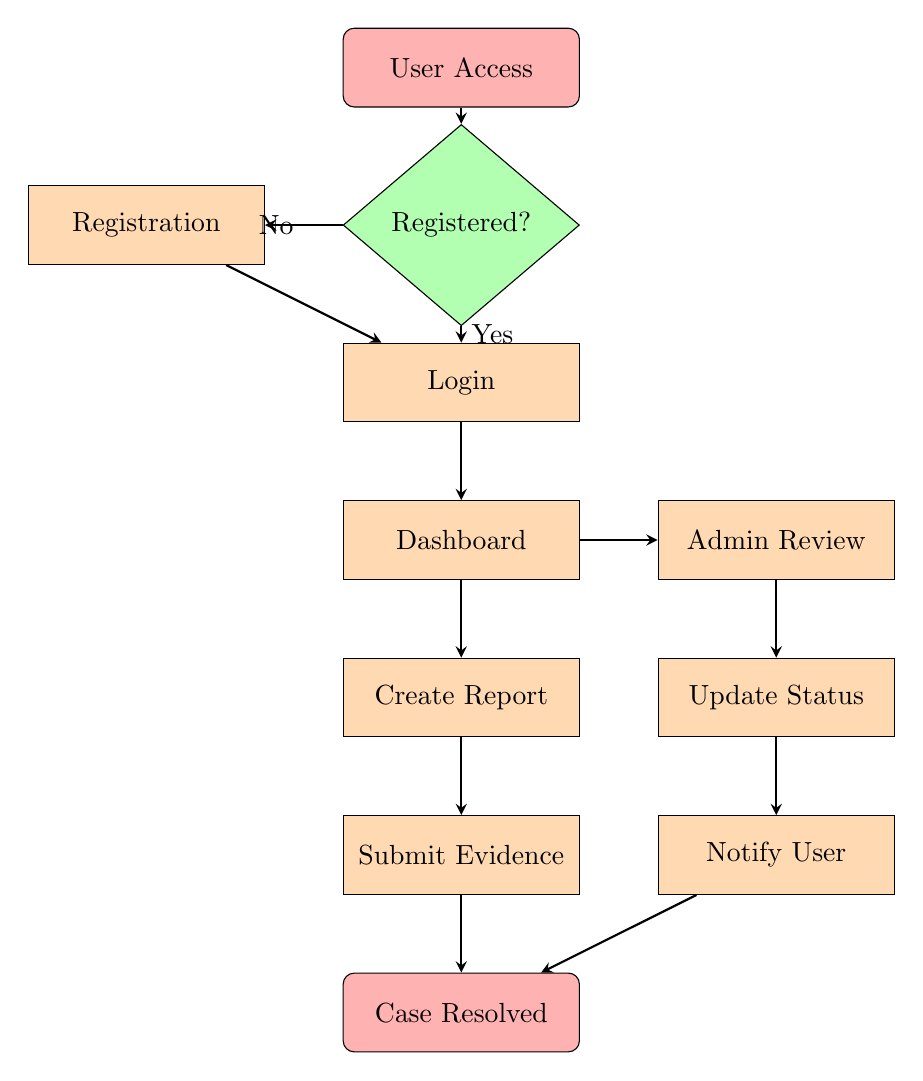
\begin{tikzpicture}[node distance=2cm, auto]
% Define styles
\tikzstyle{startstop} = [rectangle, rounded corners, minimum width=3cm, minimum height=1cm, text centered, draw=black, fill=red!30]
\tikzstyle{process} = [rectangle, minimum width=3cm, minimum height=1cm, text centered, draw=black, fill=orange!30]
\tikzstyle{decision} = [diamond, minimum width=3cm, minimum height=1cm, text centered, draw=black, fill=green!30]
\tikzstyle{arrow} = [thick,->,>=stealth]

% Place nodes
\node (start) [startstop] {User Access};
\node (register) [decision, below of=start] {Registered?};
\node (signup) [process, left of=register, xshift=-2cm] {Registration};
\node (login) [process, below of=register] {Login};
\node (dashboard) [process, below of=login] {Dashboard};
\node (report) [process, below of=dashboard] {Create Report};
\node (submit) [process, below of=report] {Submit Evidence};
\node (admin) [process, right of=dashboard, xshift=2cm] {Admin Review};
\node (status) [process, below of=admin] {Update Status};
\node (notify) [process, below of=status] {Notify User};
\node (end) [startstop, below of=submit] {Case Resolved};

% Draw arrows
\draw [arrow] (start) -- (register);
\draw [arrow] (register) -- node[anchor=east] {No} (signup);
\draw [arrow] (signup) -- (login);
\draw [arrow] (register) -- node[anchor=west] {Yes} (login);
\draw [arrow] (login) -- (dashboard);
\draw [arrow] (dashboard) -- (report);
\draw [arrow] (report) -- (submit);
\draw [arrow] (dashboard) -- (admin);
\draw [arrow] (admin) -- (status);
\draw [arrow] (status) -- (notify);
\draw [arrow] (submit) -- (end);
\draw [arrow] (notify) -- (end);
\end{tikzpicture}
\caption{CyberGuard System Workflow}
\label{fig:workflow}
\end{figure}

\subsection{Database Design}

The database schema is designed to efficiently store and retrieve cybercrime reporting data while maintaining referential integrity and supporting complex queries for administrative functions. The schema consists of several interconnected tables that represent different aspects of the cybercrime reporting process.

The Users table serves as the central repository for user account information, storing essential details such as names, email addresses, phone numbers, and encrypted passwords. The table includes role-based access control fields that distinguish between regular users and administrative users, enabling appropriate access restrictions throughout the application.

The Reports table contains the core cybercrime incident data, including incident descriptions, categorizations, evidence file references, and status tracking information. This table maintains foreign key relationships with the Users table to associate reports with their submitters while preserving data integrity.

The Tips table stores educational content and prevention advice that helps users protect themselves from cyber threats. This content management system enables administrators to maintain current and relevant cybersecurity information for public access.

Additional supporting tables handle session management, audit logging, and system configuration, providing comprehensive data management capabilities for all system operations.

\subsection{Security Architecture}

Security considerations permeate every aspect of the CyberGuard system design, reflecting the sensitive nature of cybercrime reporting data and the need to protect both user privacy and system integrity. The security architecture implements multiple layers of protection, following industry best practices and established security frameworks.

Authentication mechanisms utilize bcrypt hashing for password storage \citep{bcrypt2023hashing}, ensuring that user credentials remain protected even in the event of database compromise. Session management employs secure, HTTP-only cookies with appropriate expiration policies to prevent session hijacking and unauthorized access.

Input validation and sanitization procedures are implemented at multiple levels, following OWASP security guidelines \citep{owasp2023top10}, including client-side validation for user experience enhancement and server-side validation for security enforcement. These measures protect against common web application vulnerabilities such as SQL injection, cross-site scripting (XSS), and cross-site request forgery (CSRF).

File upload security measures include file type validation, size restrictions, and secure storage mechanisms that prevent malicious file execution while preserving evidence integrity. Uploaded files are stored in isolated directories with restricted access permissions and are served through controlled endpoints that prevent direct file system access.

\section{Implementation Details}

\subsection{Backend Development}

The backend implementation leverages the Node.js runtime environment and Express.js framework to create a robust, scalable server-side application. The modular architecture separates different functional areas into distinct modules, facilitating code organization, testing, and maintenance.

The authentication module implements comprehensive user management functionality, including registration, login, logout, and session management. Password security utilizes the bcrypt library with appropriate salt rounds to ensure strong protection against rainbow table and brute force attacks. Session management employs the express-session middleware with secure configuration options.

The reporting module handles all aspects of cybercrime incident reporting, from initial form submission through case resolution. This module implements complex business logic for incident categorization, evidence handling, and status tracking. File upload functionality utilizes the Multer middleware \citep{multer2023upload} with custom configuration for security and storage management.

The administrative module provides comprehensive case management capabilities for authorized users. This includes report review functionality, status updates, user communication, and system analytics. Role-based access control ensures that administrative functions are only accessible to authorized personnel.

Database interaction is abstracted through custom model classes that provide consistent interfaces for data operations while supporting multiple database systems. These models implement proper error handling, transaction management, and query optimization to ensure reliable data operations.

\subsection{Frontend Development}

The frontend implementation emphasizes user experience, accessibility, and responsive design to ensure that the application serves users effectively across various devices and usage contexts. The presentation layer utilizes EJS templating engine \citep{ejs2023templating} and modern web standards to deliver optimal functionality.

The user interface design follows contemporary web design principles, incorporating clean layouts, intuitive navigation, and clear visual hierarchies. The color scheme and typography choices reflect the serious nature of cybercrime reporting while maintaining approachability for users who may be stressed or unfamiliar with technology.

Form design receives particular attention, as the quality of incident reporting depends heavily on users' ability to provide comprehensive, accurate information. Forms include helpful guidance text, validation feedback, and progressive disclosure techniques to manage complexity while ensuring completeness.

Responsive design implementation using Tailwind CSS \citep{tailwind2023css} ensures that all functionality remains accessible and usable across different screen sizes and input methods. The mobile-first approach prioritizes essential functionality for smaller screens while enhancing the experience on larger displays.

JavaScript functionality enhances user interactions through client-side validation, dynamic form behavior, and improved navigation. The implementation follows progressive enhancement principles, ensuring that core functionality remains available even when JavaScript is disabled or unavailable.

\subsection{Database Implementation}

The database implementation supports both MySQL and PostgreSQL systems through a unified abstraction layer that enables deployment flexibility while maintaining consistent functionality. The schema design optimizes for both transactional operations and analytical queries required for administrative functions.

Table structures implement appropriate indexing strategies to ensure efficient query performance as the system scales. Primary keys, foreign keys, and unique constraints maintain data integrity while supporting complex relational queries. Proper normalization reduces data redundancy while preserving query efficiency.

Connection pooling and transaction management ensure reliable database operations under varying load conditions. The implementation includes comprehensive error handling and recovery mechanisms to maintain system stability during database connectivity issues or high-load scenarios.

Data migration scripts facilitate schema updates and system maintenance, enabling smooth deployment of new features and bug fixes. Version control for database schemas ensures consistency across development, testing, and production environments.

\section{Features and Functionality}

\subsection{User Registration and Authentication}

The user registration system provides a streamlined onboarding process that balances security requirements with user convenience. New users can create accounts by providing essential information including full name, email address, and secure password. Optional phone number collection enables additional communication channels for case updates and security notifications.

Email validation ensures that users provide legitimate contact information while preventing automated account creation. Password strength requirements enforce minimum security standards without creating excessive barriers to registration. The system provides clear feedback on password requirements and validation status to guide users through the registration process.

Account activation mechanisms could be implemented to verify email addresses and prevent abuse, though the current implementation prioritizes immediate access to encourage reporting. Future enhancements might include email verification workflows and additional identity verification options for enhanced security.

The login system implements secure authentication practices including protection against brute force attacks, session management, and secure password handling. Users receive clear feedback on authentication failures while security measures prevent information disclosure that could assist attackers.

\subsection{Cybercrime Reporting System}

The core reporting functionality enables users to document cybercrime incidents comprehensively while providing guidance and support throughout the process. The reporting interface guides users through structured data collection that ensures all necessary information is captured for effective investigation.

Incident categorization helps users identify the appropriate classification for their experiences while enabling systematic organization of reports for administrative review. Categories include common cybercrime types such as phishing, identity theft, financial fraud, cyberbullying, ransomware, and social media fraud, with an "other" option for incidents that don't fit standard categories.

The description interface encourages detailed incident documentation while providing guidance on important information to include. Users can describe the sequence of events, identify potential evidence, and specify any immediate concerns or ongoing threats. Rich text editing capabilities enable proper formatting and organization of complex incident descriptions.

Evidence attachment functionality allows users to submit supporting documentation, screenshots, and other digital evidence that may assist in investigation. File upload security measures ensure that malicious files cannot compromise system security while preserving the integrity of legitimate evidence submissions.

Report tracking capabilities provide users with visibility into case progress and administrative actions. Status updates, administrative responses, and case resolution information help users understand the investigation process and outcomes.

\subsection{Administrative Dashboard}

The administrative interface provides comprehensive case management capabilities for authorized personnel responsible for reviewing and investigating cybercrime reports. The dashboard presents key metrics and recent activity to enable efficient workload management and priority identification.

Statistical displays show total reports, pending cases, cases under review, and resolved cases, providing administrators with immediate insight into system activity and workload distribution. Trend analysis capabilities help identify patterns in cybercrime reporting that may indicate emerging threats or seasonal variations.

Report management functionality enables administrators to review submitted reports, update case statuses, and communicate with report submitters. Detailed report views present all submitted information in organized formats that facilitate efficient review and decision-making.

Status update capabilities allow administrators to progress cases through defined workflows while maintaining audit trails of all administrative actions. Standardized status categories ensure consistent case handling while providing clear communication to report submitters about case progress.

Communication tools enable administrators to request additional information from report submitters, provide updates on investigation progress, and communicate case resolutions. These tools maintain professional communication standards while ensuring that sensitive information is handled appropriately.

\subsection{Educational Resources}

The tips and prevention section provides valuable cybersecurity education to help users protect themselves from cyber threats. This educational component serves both reactive and proactive purposes, helping current victims understand their situations while preventing future incidents.

Content organization categorizes information by threat type, target audience, and complexity level to ensure that users can find relevant information quickly. Topics cover common scam techniques, safe online practices, password security, social media privacy, and incident response procedures.

Regular content updates ensure that educational materials remain current with evolving threat landscapes and emerging attack techniques. Administrative tools enable authorized users to add, edit, and organize educational content without requiring technical expertise.

Accessibility features ensure that educational content is available to users with varying abilities and technical skill levels. Clear language, visual aids, and structured presentation make complex cybersecurity concepts understandable to general audiences.

\section{Testing and Quality Assurance}

\subsection{Testing Methodology}

The testing approach for CyberGuard encompasses multiple testing levels and methodologies to ensure comprehensive quality assurance. The testing strategy addresses functional requirements, security considerations, performance characteristics, and user experience factors that are critical for a cybercrime reporting system.

Unit testing focuses on individual components and functions, verifying that each piece of code performs its intended function correctly under various input conditions. The Node.js ecosystem provides excellent testing frameworks such as Jest and Mocha that facilitate comprehensive unit test development and execution.

Integration testing verifies that different system components work together correctly, particularly focusing on database interactions, API endpoints, and authentication workflows. These tests ensure that data flows correctly between system layers and that error handling mechanisms function properly under various failure scenarios.

System testing evaluates the complete application functionality from end-user perspectives, verifying that all features work correctly in realistic usage scenarios. This testing level includes complete user workflows from registration through report submission and case resolution.

User acceptance testing involves stakeholders and potential users in evaluating system usability, functionality, and overall effectiveness. This testing approach helps identify usability issues and ensures that the system meets real-world requirements for cybercrime reporting.

\subsection{Security Testing}

Security testing receives particular emphasis given the sensitive nature of cybercrime reporting data and the potential consequences of security breaches. The security testing approach addresses common web application vulnerabilities as well as specific threats relevant to cybercrime reporting systems.

Authentication and authorization testing verifies that access controls function correctly under various scenarios, including attempts to access unauthorized resources, session manipulation, and privilege escalation attacks. These tests ensure that user data remains protected and that administrative functions are properly restricted.

Input validation testing examines system responses to malicious or malformed input data, including SQL injection attempts, cross-site scripting payloads, and file upload attacks. Comprehensive input validation testing helps identify potential vulnerabilities before system deployment.

Session management testing evaluates the security of user sessions, including session creation, maintenance, and termination processes. These tests verify that sessions cannot be hijacked or manipulated by unauthorized parties.

Data protection testing ensures that sensitive information is properly encrypted, stored securely, and transmitted safely. This includes testing password hashing mechanisms, database security measures, and secure communication protocols.

\subsection{Performance Testing}

Performance testing evaluates system behavior under various load conditions to ensure that the application can handle expected usage levels while maintaining acceptable response times and resource utilization. Performance considerations are particularly important for public-facing systems that may experience variable and unpredictable usage patterns.

Load testing simulates normal usage conditions to establish baseline performance characteristics and identify potential bottlenecks. These tests help determine appropriate hardware requirements and identify optimization opportunities.

Stress testing evaluates system behavior under extreme load conditions to identify failure points and ensure graceful degradation when resources are exhausted. Understanding system limits helps in capacity planning and incident response preparation.

Database performance testing focuses on query optimization, connection management, and data retrieval efficiency. Given the importance of data operations in cybercrime reporting, database performance directly impacts user experience and system scalability.

Frontend performance testing evaluates page load times, resource utilization, and user interface responsiveness across different devices and network conditions. Mobile performance receives particular attention given the increasing prevalence of mobile internet usage.

\section{Deployment and Infrastructure}

\subsection{Cloud Deployment Strategy}

The deployment strategy for CyberGuard emphasizes reliability, security, and cost-effectiveness while ensuring that the system remains accessible to users regardless of their geographic location or technical infrastructure. Cloud deployment provides the scalability and reliability necessary for a public service application \citep{render2023deployment}.

Platform selection considers factors such as security certifications, compliance capabilities, geographic distribution, and cost structures. Render.com was selected as the primary deployment platform due to its developer-friendly approach, integrated database services, and competitive pricing for small to medium-scale applications.

The deployment architecture utilizes containerization principles to ensure consistent behavior across development, testing, and production environments. This approach simplifies deployment processes while reducing the likelihood of environment-specific issues.

Automated deployment pipelines integrate with version control systems to enable continuous integration and deployment practices. These pipelines include automated testing, security scanning, and deployment verification to ensure that only properly tested code reaches production environments.

\subsection{Database Deployment}

Database deployment considerations address data security, backup procedures, performance optimization, and disaster recovery requirements. The database contains sensitive cybercrime reporting data that requires appropriate protection measures and availability guarantees.

PostgreSQL deployment on Render.com provides managed database services that include automated backups, security updates, and performance monitoring. This managed approach reduces operational overhead while ensuring that database administration follows industry best practices.

Database security configuration includes encryption at rest and in transit, access control restrictions, and audit logging capabilities. These measures ensure that sensitive data remains protected throughout its lifecycle.

Backup and recovery procedures ensure that cybercrime reporting data can be restored in the event of system failures or data corruption. Regular backup testing verifies that recovery procedures function correctly and that data integrity is maintained.

\subsection{Monitoring and Maintenance}

System monitoring provides visibility into application performance, security events, and user activity to enable proactive maintenance and incident response. Comprehensive monitoring helps identify issues before they impact users and provides data for system optimization.

Application performance monitoring tracks response times, error rates, and resource utilization to identify performance trends and potential issues. This monitoring helps ensure that the system continues to meet performance expectations as usage grows.

Security monitoring includes intrusion detection, authentication monitoring, and suspicious activity identification. Given the sensitive nature of cybercrime reporting, security monitoring helps protect both user data and system integrity.

Log management systems collect, analyze, and retain system logs for troubleshooting, security analysis, and compliance purposes. Proper log management enables effective incident response and provides audit trails for administrative actions.

\section{Results and Analysis}

\subsection{System Performance Metrics}

The deployed CyberGuard system demonstrates strong performance characteristics across key metrics that impact user experience and system reliability. Performance analysis encompasses response times, throughput capabilities, resource utilization, and scalability characteristics under various load conditions.

Response time measurements show that the application consistently delivers page loads within acceptable timeframes, with average response times under 2 seconds for most operations. Database queries execute efficiently due to proper indexing and query optimization, contributing to overall system responsiveness.

Throughput testing indicates that the system can handle concurrent users effectively, with performance degradation remaining minimal under normal load conditions. The Node.js event-driven architecture contributes to efficient handling of concurrent connections and requests.

Resource utilization monitoring shows efficient use of server resources, with memory and CPU usage remaining within acceptable ranges during normal operations. The lightweight nature of the Node.js runtime contributes to efficient resource utilization.

Scalability analysis suggests that the current architecture can accommodate growth in user base and reporting volume through horizontal scaling approaches. Cloud deployment facilitates scaling operations when increased capacity becomes necessary.

\subsection{User Experience Analysis}

User experience evaluation encompasses usability testing results, accessibility assessments, and feedback from stakeholders who have interacted with the system. The user-centered design approach prioritizes ease of use and accessibility for users who may be experiencing stress or unfamiliarity with technology.

Usability testing reveals that users can successfully complete core tasks such as account registration, report submission, and status checking without significant difficulty. The intuitive interface design and clear navigation contribute to positive user experiences.

Accessibility testing confirms that the application meets web accessibility standards, ensuring that users with disabilities can access and use the system effectively. Proper semantic markup, keyboard navigation support, and screen reader compatibility contribute to inclusive design.

Mobile usability testing demonstrates that the responsive design approach successfully adapts the interface for smaller screens while maintaining full functionality. Mobile users can complete all essential tasks without requiring desktop access.

Form usability analysis shows that the structured approach to incident reporting helps users provide comprehensive information while minimizing cognitive load. Progressive disclosure and helpful guidance text contribute to successful form completion rates.

\subsection{Security Assessment Results}

Security assessment encompasses vulnerability testing, penetration testing results, and compliance with security best practices relevant to web applications handling sensitive data. The security-first approach to development helps ensure that user data remains protected.

Vulnerability scanning reveals no critical security issues in the deployed application, with proper implementation of input validation, authentication mechanisms, and access controls. Regular security updates and monitoring help maintain security posture over time.

Authentication security testing confirms that password hashing, session management, and access control mechanisms function correctly and resist common attack techniques. The implementation follows established security frameworks such as NIST Cybersecurity Framework \citep{nist2023framework} and CISA guidelines \citep{cisa2023guidelines}.

Data protection assessment verifies that sensitive information is properly encrypted, stored securely, and transmitted safely. Database security measures and secure communication protocols contribute to comprehensive data protection.

File upload security testing confirms that evidence attachment functionality properly validates file types and prevents malicious file execution while preserving legitimate evidence integrity.

\section{Challenges and Solutions}

\subsection{Technical Challenges}

The development of CyberGuard encountered several technical challenges that required innovative solutions and careful consideration of trade-offs between functionality, security, and usability. These challenges provided valuable learning opportunities and contributed to a more robust final system.

Database abstraction presented complexity in supporting both MySQL and PostgreSQL while maintaining consistent functionality and performance. The solution involved creating a unified model layer that abstracts database-specific operations while preserving the ability to optimize for specific database features when necessary.

File upload security required balancing evidence preservation needs with system security requirements. The implemented solution includes comprehensive file validation, secure storage mechanisms, and controlled access procedures that protect system integrity while preserving evidence value.

Responsive design implementation across diverse devices and screen sizes required careful consideration of information hierarchy and interaction patterns. The mobile-first approach and progressive enhancement techniques ensure consistent functionality across platforms.

Performance optimization under varying load conditions required careful analysis of bottlenecks and implementation of appropriate caching and optimization strategies. Database query optimization and efficient resource management contribute to consistent performance.

\subsection{User Experience Challenges}

Creating an interface that serves both technical and non-technical users while handling sensitive cybercrime reporting presented unique user experience challenges. The solution approach emphasized clarity, guidance, and emotional sensitivity in design decisions.

Form complexity management required balancing comprehensive data collection with user-friendly interfaces. The implemented solution uses progressive disclosure, helpful guidance text, and clear validation feedback to manage complexity while ensuring completeness.

Status communication presented challenges in explaining complex investigation processes in terms that users can understand. The solution involves clear status categories, explanatory text, and regular communication to keep users informed about case progress.

Accessibility requirements demanded careful attention to users with varying abilities and technical skill levels. The implementation includes semantic markup, keyboard navigation support, and clear visual design that serves diverse user needs.

Trust and credibility establishment required design decisions that convey professionalism and security while remaining approachable for users who may be experiencing stress or trauma. The visual design and communication tone balance these requirements effectively.

\subsection{Deployment Challenges}

Deployment to cloud infrastructure presented challenges related to environment configuration, security setup, and performance optimization. The solutions developed provide a foundation for reliable, scalable system operation.

Environment configuration management required ensuring consistency between development, testing, and production environments while maintaining security. The solution involves containerization principles and automated deployment procedures that reduce configuration drift.

Database migration and setup required careful planning to ensure data integrity and security during deployment processes. The implemented procedures include comprehensive testing and rollback capabilities to minimize deployment risks.

Security configuration in cloud environments required understanding platform-specific security features and best practices. The implementation leverages platform security capabilities while maintaining application-level security measures.

Performance optimization for cloud deployment required understanding platform characteristics and optimization opportunities. The solution includes appropriate resource allocation, caching strategies, and monitoring procedures.

\section{Future Enhancements}

\subsection{Feature Expansion}

The current CyberGuard implementation provides a solid foundation for cybercrime reporting that can be enhanced with additional features to better serve users and administrators. Future development priorities focus on improving user experience, expanding functionality, and integrating with external systems.

Email notification systems would provide automated updates to users about case progress, reducing the need for manual status checking while keeping users informed about important developments. Integration with email services and template management systems would enable professional, timely communication.

Real-time chat support functionality would provide immediate assistance to users who need help with reporting processes or have questions about cybersecurity. Integration with customer service platforms and chatbot technologies could provide scalable support capabilities.

Advanced search and filtering capabilities would help administrators manage large volumes of reports more efficiently. Implementation of full-text search, advanced filtering options, and data visualization tools would improve administrative productivity.

Mobile application development would provide native mobile interfaces that could offer enhanced functionality such as camera integration for evidence collection, push notifications for status updates, and offline capability for areas with limited connectivity.

Multi-language support would expand accessibility to non-English speaking users, requiring internationalization framework implementation, translation management, and cultural adaptation of user interfaces and communication.

\subsection{Technical Improvements}

Technical enhancement opportunities focus on performance optimization, security strengthening, and architectural improvements that would support system growth and evolution. These improvements would enhance both user experience and system maintainability.

API development would enable integration with external systems such as law enforcement databases, cybersecurity threat intelligence platforms, and mobile applications. RESTful API design and documentation would facilitate third-party integrations.

Advanced analytics capabilities would provide insights into cybercrime trends, reporting patterns, and system usage that could inform policy decisions and resource allocation. Integration with business intelligence tools and data visualization platforms would enable comprehensive analysis.

Microservices architecture migration would improve system scalability, maintainability, and deployment flexibility. Breaking the monolithic application into focused services would enable independent scaling and development of different system components.

Enhanced security measures including two-factor authentication, advanced threat detection, and security information and event management (SIEM) integration would strengthen protection against evolving cyber threats.

Performance optimization through caching layers, content delivery networks, and database optimization would improve user experience and reduce infrastructure costs as the system scales.

\subsection{Integration Opportunities}

Integration with external systems and services would enhance CyberGuard's value proposition and effectiveness in addressing cybercrime. These integrations would leverage existing infrastructure and expertise while expanding system capabilities.

Law enforcement system integration would enable direct case forwarding to appropriate agencies, reducing manual processing and improving response times. Integration would require careful attention to security, privacy, and jurisdictional requirements.

Cybersecurity threat intelligence integration would provide real-time information about emerging threats, enabling proactive user education and improved incident categorization. Integration with threat intelligence platforms would enhance system knowledge and effectiveness.

Social media platform integration could enable automated detection and reporting of cybercrime incidents, particularly for cases involving social media fraud or cyberbullying. API integration with major platforms would facilitate evidence collection and incident documentation.

Financial institution integration could streamline reporting of financial fraud cases while enabling real-time fraud detection and prevention. Secure integration with banking systems would require careful attention to regulatory compliance and data protection.

Educational institution partnerships could facilitate cybersecurity education and awareness programs while providing research opportunities for cybercrime analysis and prevention strategy development.

\section{Conclusion}

\subsection{Project Summary}

The CyberGuard project successfully demonstrates the development and deployment of a comprehensive cybercrime reporting system that addresses critical needs in digital security and law enforcement. The application provides an accessible, secure platform for citizens to report cybercrime incidents while offering administrative tools for case management and user education.

The technical implementation showcases modern web development practices, security-first design principles, and user-centered development approaches. The system architecture supports scalability, maintainability, and security requirements while delivering excellent user experience across diverse devices and usage contexts.

Key achievements include successful deployment on cloud infrastructure, implementation of robust security measures, creation of intuitive user interfaces, and development of comprehensive administrative capabilities. The system demonstrates that complex cybercrime reporting requirements can be addressed through thoughtful design and careful implementation.

The project provides valuable insights into the challenges and opportunities in developing public service applications that handle sensitive data while serving diverse user populations. The solutions developed and lessons learned contribute to the broader knowledge base for cybersecurity application development.

\subsection{Impact and Significance}

The CyberGuard system addresses a critical gap in cybercrime reporting infrastructure by providing an accessible, user-friendly platform that encourages reporting while supporting effective case management. The impact extends beyond individual users to contribute to broader cybersecurity awareness and law enforcement effectiveness.

For individual users, the system provides a safe, confidential way to report cybercrime incidents while accessing educational resources that help prevent future victimization. The user-centered design approach ensures that the system serves users effectively regardless of their technical expertise or emotional state.

For administrators and law enforcement, the system provides efficient tools for managing cybercrime reports, tracking case progress, and communicating with victims. The structured data collection and organization capabilities support more effective investigation and response procedures.

For the broader community, the system contributes to cybersecurity awareness and education while providing data that can inform policy decisions and resource allocation. The educational components help build community resilience against cyber threats.

The technical contributions include demonstration of security best practices, responsive design implementation, and cloud deployment strategies that can inform similar projects. The open-source nature of many components enables knowledge sharing and collaborative improvement.

\subsection{Lessons Learned}

The development process provided valuable insights into the complexities of building public service applications that handle sensitive data while serving diverse user populations. These lessons inform future development efforts and contribute to best practices for similar projects.

User-centered design proves essential for applications serving stressed or traumatized users who may have limited technical expertise. Extensive user research, iterative design processes, and accessibility considerations are crucial for creating effective interfaces.

Security considerations must be integrated throughout the development process rather than added as an afterthought. The sensitive nature of cybercrime reporting data requires comprehensive security measures that protect both user privacy and system integrity.

Cloud deployment offers significant advantages for public service applications, including scalability, reliability, and cost-effectiveness. However, successful cloud deployment requires careful planning, security configuration, and ongoing monitoring.

Comprehensive testing across multiple dimensions including functionality, security, performance, and usability is essential for applications that serve critical public needs. Automated testing procedures and continuous integration practices support reliable system operation.

Documentation and knowledge transfer are crucial for long-term system sustainability. Comprehensive documentation enables effective maintenance, enhancement, and knowledge sharing that extends system value over time.

\subsection{Future Directions}

The CyberGuard project establishes a foundation for continued development and enhancement that can adapt to evolving cybercrime threats and user needs. Future directions focus on expanding functionality, improving integration capabilities, and enhancing user experience.

Immediate priorities include implementing user feedback from initial deployment, addressing any identified issues or limitations, and optimizing system performance based on actual usage patterns. Continuous improvement processes ensure that the system evolves to meet user needs effectively.

Medium-term development focuses on feature expansion including mobile applications, advanced analytics, and integration with external systems. These enhancements would significantly expand system capabilities and value proposition.

Long-term vision includes establishing CyberGuard as a comprehensive cybersecurity platform that serves not only individual reporting needs but also contributes to broader cybersecurity research, policy development, and community education initiatives.

Research opportunities include analysis of cybercrime reporting patterns, effectiveness of different prevention strategies, and user behavior studies that could inform both system improvements and broader cybersecurity policy decisions.

The project demonstrates that thoughtful application of modern web technologies can address complex social problems while providing valuable learning opportunities for developers, researchers, and policymakers working to improve cybersecurity outcomes for all citizens.

\section{Works Cited}

\begin{thebibliography}{99}

\bibitem{bcrypt2023hashing}
Bcrypt Development Team. "Bcrypt Password Hashing Library." \textit{GitHub}, 2023, github.com/kelektiv/node.bcrypt.js. Accessed 24 Nov. 2023.

\bibitem{cisa2023guidelines}
Cybersecurity and Infrastructure Security Agency. "Cybersecurity Best Practices." \textit{Department of Homeland Security}, 2023, cisa.gov/cybersecurity-best-practices. Accessed 24 Nov. 2023.

\bibitem{ejs2023templating}
EJS Development Team. "Embedded JavaScript Templates." \textit{EJS Official Documentation}, 2023, ejs.co. Accessed 24 Nov. 2023.

\bibitem{expressjs2023security}
Express.js Team. "Express.js Security Best Practices." \textit{Express.js Official Documentation}, 2023, expressjs.com/en/advanced/best-practice-security.html. Accessed 24 Nov. 2023.

\bibitem{fbi2023cybercrime}
FBI Internet Crime Complaint Center. \textit{Internet Crime Report 2023}. Federal Bureau of Investigation, 2023.

\bibitem{ic3report2023}
Internet Crime Complaint Center. "Annual Report 2023." \textit{IC3.gov}, FBI, 2023, ic3.gov/Media/PDF/AnnualReport/2023_IC3Report.pdf. Accessed 24 Nov. 2023.

\bibitem{mdn2023responsive}
Mozilla Developer Network. "Responsive Web Design." \textit{MDN Web Docs}, Mozilla Foundation, 2023, developer.mozilla.org/en-US/docs/Learn/CSS/CSS_layout/Responsive_Design. Accessed 24 Nov. 2023.

\bibitem{morgan2020cybersecurity}
Morgan, Steve. \textit{Cybersecurity Ventures 2021 Official Annual Cybercrime Report}. Cybersecurity Ventures, 2020.

\bibitem{multer2023upload}
Multer Development Team. "Multer File Upload Middleware." \textit{GitHub}, 2023, github.com/expressjs/multer. Accessed 24 Nov. 2023.

\bibitem{nist2023framework}
National Institute of Standards and Technology. \textit{Framework for Improving Critical Infrastructure Cybersecurity}. NIST Special Publication 800-53, Version 1.1, U.S. Department of Commerce, 2023.

\bibitem{nodejs2023performance}
Node.js Foundation. "Node.js Performance Best Practices." \textit{Node.js Official Documentation}, 2023, nodejs.org/en/docs/guides/simple-profiling. Accessed 24 Nov. 2023.

\bibitem{owasp2023top10}
OWASP Foundation. "OWASP Top 10 Web Application Security Risks." \textit{OWASP.org}, 2023, owasp.org/www-project-top-ten. Accessed 24 Nov. 2023.

\bibitem{postgresql2023security}
PostgreSQL Global Development Group. "PostgreSQL Security Documentation." \textit{PostgreSQL Official Documentation}, 2023, postgresql.org/docs/current/security.html. Accessed 24 Nov. 2023.

\bibitem{provos1999bcrypt}
Provos, Niels, and David Mazi\`{e}res. "A Future-Adaptable Password Scheme." \textit{Proceedings of the FREENIX Track: 1999 USENIX Annual Technical Conference}, USENIX Association, 1999, pp. 81-91.

\bibitem{render2023deployment}
Render Inc. "Cloud Deployment Documentation." \textit{Render Official Documentation}, 2023, render.com/docs. Accessed 24 Nov. 2023.

\bibitem{tailwind2023css}
Tailwind Labs. "Tailwind CSS Documentation." \textit{Tailwind CSS Official Site}, 2023, tailwindcss.com/docs. Accessed 24 Nov. 2023.

\end{thebibliography}

\end{document}